\section{Radiance Fields}

Radiance fields represent a revolutionary approach to 3D scene representation and rendering, offering extreme photorealism compared to traditional computer graphics methods such as meshes. This approach builds on foundational work in light fields and volumetric rendering, which demonstrated the feasibility of capturing complex scenes without explicit geometric modeling. Light fields \citep{lum1994light} represented scenes as 4D functions of light rays, capturing both spatial and directional variation of light. This work demonstrated the possibility of representing complex scenes without explicit geometry, being significantly different from traditional mesh-based approaches. The success of light fields in capturing view-dependent effects and complex light transport phenomena laid the groundwork for future developments in the field \citep{levoy1996light}.






\subsection{Theoretical Foundation}

At its core, a radiance field is a continuous function that maps every point in 3D space and viewing direction to a color and density value. This mathematical representation enables the modeling of intricate light transport phenomena, including scattering, absorption, view-dependent effects, and complex material interactions. Formally, a radiance field is defined as a function \( f \) that takes a 3D position \( \mathbf{x} \in \mathbb{R}^3 \) and a viewing direction \( \mathbf{d} \in \mathbb{S}^2 \) and outputs a color \( \mathbf{c} \) and density \( \sigma \):

\begin{equation}
f: (\mathbf{x}, \mathbf{d}) \mapsto (\mathbf{c}, \sigma)
\end{equation}

This formulation allows radiance fields to encode both the geometry and appearance of a scene in a unified framework, bypassing the need for explicit surface representations.





\subsection{Creation Methods}

One of the most significant advantages of radiance fields over meshes is their ability to be reconstructed directly from real-world data, such as images or videos. Unlike traditional mesh-based approaches, which often require manual modeling or complex reconstruction pipelines, radiance fields can be learned from a set of calibrated photographs. The learning process involves optimizing a neural network to minimize the difference between rendered views and the ground truth images:

\begin{equation}
\text{minimize } \mathcal{L} = \sum_{i=1}^N \|R_i - \hat{R}_i\|_2^2
\end{equation}

where \( R_i \) is the ground truth image from camera view \( i \), and \( \hat{R}_i \) is the corresponding rendered view from the radiance field. Early approaches to radiance fields relied on explicit representations, such as voxel grids or point clouds, to store scene information. However, these methods struggled to capture fine details and view-dependent effects efficiently, limiting their practicality for photorealistic rendering.

The introduction of neural networks marked a turning point in radiance field research. By leveraging the expressive power of neural networks, researchers were able to approximate the continuous radiance field function in a compact and efficient manner. This data-driven approach eliminates the need for manual intervention, enabling the automatic reconstruction of highly detailed and photorealistic scenes from real-world observations \citep{izadi2011kinect}.




\subsection{Radiance Field Techniques}

The field of radiance fields has seen rapid advancements, with numerous techniques emerging to improve efficiency, quality, and applicability. Two of the most prominent methods are Neural Radiance Fields (NeRF) and Gaussian Splatting.

\subsubsection{Neural Radiance Fields (NeRF)}

NeRF \citep{mildenhall2020nerf} revolutionized 3D scene representation by leveraging neural networks to model radiance fields implicitly. Instead of explicitly storing scene data, such as meshes or point clouds, NeRF employs a neural network \( f_\theta \) with learnable parameters \( \theta \) to map 3D positions \( \mathbf{x} = (x, y, z) \) and 2D viewing directions \( \mathbf{d} = (\theta, \phi) \) to color \( \mathbf{c} = (r, g, b) \) and density \( \sigma \):

\begin{equation}
 f_\theta : (\mathbf{x}, \mathbf{d}) \mapsto (\mathbf{c}, \sigma)
\end{equation}

The network \( f_\theta \) is trained using gradient-based optimization to minimize the difference between rendered images and ground truth images. This process allows the network to encode both the geometry (via density \( \sigma \)) and appearance (via color \( \mathbf{c} \)) of the scene within its weights. The optimization is performed using a dataset of images with known camera parameters (position, rotation, fov ...), enabling the network to learn a 3D representation of the scene.

\subsubsection*{Training Process}
The training process involves the following key steps:

\begin{enumerate}
    \item \textbf{Ray Sampling}: For each training image, a set of camera rays is generated, corresponding to the pixels in the image. Each ray \( \mathbf{r}(t) = \mathbf{o} + t\mathbf{d} \) is sampled at multiple points along its path, where \( \mathbf{o} \) is the ray origin (camera position), \( \mathbf{d} \) is the ray direction, and \( t \) represents the distance along the ray.

    \item \textbf{Volume Rendering}: For each sampled point \( \mathbf{x}_i = \mathbf{r}(t_i) \), the network predicts the color \( \mathbf{c}_i \) and density \( \sigma_i \). These values are used to approximate the pixel color \( C(\mathbf{r}) \) via volumetric rendering, as described by \ref{pre::volumetric-render-equation}.

    \item \textbf{Loss Computation}: The rendered color \( C(\mathbf{r}) \) is compared to the ground truth pixel color \( C_{\text{gt}}(\mathbf{r}) \) using a photometric loss, typically the mean squared error (MSE):

\begin{equation}
 \mathcal{L} = \frac{1}{N} \sum_{\mathbf{r}} \| C(\mathbf{r}) - C_{\text{gt}}(\mathbf{r}) \|^2
\end{equation}

Here, \( N \) is the total number of rays sampled during training. The loss measures the discrepancy between the rendered and ground truth images, driving the network to improve its predictions.

    \item \textbf{Gradient-Based Optimization}: The parameters \( \theta \) of the network are updated using gradient descent or a variant (e.g., Adam optimizer) to minimize the loss. The gradients are computed via backpropagation, leveraging the differentiability of the volumetric rendering process.
\end{enumerate}

\subsubsection*{Rendering}

Rendering in Neural Radiance Fields (NeRF) is achieved through a process known as \textit{volumetric rendering}. This technique simulates the way light interacts with a 3D scene by integrating color and density along camera rays. For a given camera ray \( \mathbf{r}(t) = \mathbf{o} + t\mathbf{d} \), where \( \mathbf{o} \) is the ray's origin, \( \mathbf{d} \) is its direction, and \( t \) represents the distance along the ray, the color \( C(\mathbf{r}) \) is computed as follows:

\begin{equation}
C(\mathbf{r}) = \int_{t_n}^{t_f} T(t)\sigma(\mathbf{r}(t))\mathbf{c}(\mathbf{r}(t), \mathbf{d}) \, dt
\label{pre::volumetric-render-equation}
\end{equation}

Here, \( t_n \) and \( t_f \) denote the near and far bounds of the ray, respectively. The function \( \sigma(\mathbf{r}(t)) \) represents the volume density at point \( \mathbf{r}(t) \), which determines how much light is absorbed or scattered at that location. The function \( \mathbf{c}(\mathbf{r}(t), \mathbf{d}) \) represents the color emitted at \( \mathbf{r}(t) \) in the direction \( \mathbf{d} \), capturing view-dependent effects such as reflections and specular highlights.

The term \( T(t) \), known as the \textit{accumulated transmittance}, models the attenuation of light as it travels along the ray. It is defined as:

\begin{equation}
T(t) = \exp\left(-\int_{t_n}^{t} \sigma(\mathbf{r}(s)) \, ds\right)
\end{equation}

This exponential term accounts for the probability that light reaches the point \( \mathbf{r}(t) \) without being absorbed or scattered by the volume. Intuitively, \( T(t) \) decreases as the ray passes through regions of higher density, simulating the effect of light being "blocked" by the scene's geometry.

In practice, evaluating these integrals analytically is computationally infeasible. Instead, NeRF approximates the integrals using numerical quadrature. The ray is discretized into a set of sample points \( \{t_i\} \), and the color \( C(\mathbf{r}) \) is approximated as:

\begin{equation}
C(\mathbf{r}) \approx \sum_{i=1}^N T_i \left(1 - \exp(-\sigma_i \delta_i)\right) \mathbf{c}_i
\end{equation}

where \( T_i = \exp\left(-\sum_{j=1}^{i-1} \sigma_j \delta_j\right) \) is the discrete transmittance up to sample \( i \), \( \sigma_i \) and \( \mathbf{c}_i \) are the density and color at sample \( i \), and \( \delta_i = t_{i+1} - t_i \) is the distance between adjacent samples. This formulation ensures that the rendering process is both efficient and differentiable, enabling end-to-end training of the NeRF model.

\begin{figure}[ht]
    \centering
    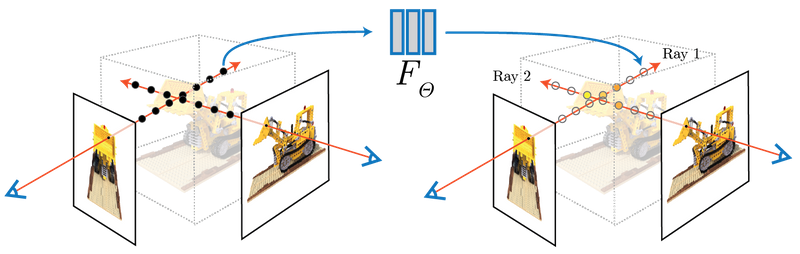
\includegraphics[width=1\linewidth]{assets/nerf_algo.png}
    \caption{NeRF training (left) and rendering (right). Rays are cast through the scene to predict color and density for training or to render novel views.}
    \label{fig:nerf-rays}
\end{figure}

In summary, NeRF's rendering pipeline combines principles from classical volume rendering with modern neural networks, resulting in a powerful framework for 3D scene reconstruction and visualization. The integration of density, color, and transmittance along camera rays allows NeRF to produce highly realistic images while maintaining computational efficiency and differentiability.

NeRF's ability to produce highly detailed and photorealistic renderings has inspired numerous extensions and optimizations, such as \textit{PlenOctrees} \citep{yu2021plenoctrees} for efficient rendering and \textit{Mip-NeRF} \citep{barron2021mipnerf} for handling multi-scale representations.


\subsubsection{Gaussian Splatting}

While NeRF achieves remarkable visual quality, its computational cost and slow rendering speeds limit its practicality for real-time applications. Gaussian Splatting \citep{kerbl2023gsplatt} addresses these limitations by representing scenes as a collection of 3D Gaussian points distributed in space. Each Gaussian is parameterized by its position, scale, rotation, and color, allowing for efficient rendering through splatting techniques. This method achieves real-time rendering speeds while maintaining high visual quality, making it particularly suitable for interactive applications \citep{zwicker2001ewa}. Gaussian Splatting forms the foundation of this thesis, as it bridges the gap between the flexibility of radiance fields and the efficiency required for practical use. The fundamentals of gaussian splatting will be explained in Section \ref{pre::gaussian-splatting}.